\documentclass[aspectratio=169]{beamer}
\usepackage{array}
\usepackage{hyperref}
\hypersetup{%
  colorlinks=true,
  linkcolor=blue,
  filecolor=blue,
  urlcolor=cyan,
}
\usepackage{graphics}
\usepackage[utf8]{inputenc}
\usepackage[T1]{fontenc}
\usepackage{listings}
\usepackage{multicol}
\usepackage{multirow}
\usepackage[absolute,overlay]{textpos}
\usepackage{setspace}
\usepackage{verbatim}
\usepackage{fancyvrb} % for verbatim centering
\usepackage{tikz}

\RequirePackage{tikz}
\title{Programowanie współbieżne}
\subtitle{Część I:\@ wprowadzenie i podstawy}
\date[11.2022]{}
\author[gralin.ski]{Adam Graliński dla C++ Friends}

\usetheme{gralmosaic}

\begin{document}

\begin{frame}
\titlepage{}
\end{frame}

\begin{frame}{Agenda}
\begin{enumerate}
  \item{} Podstawy
  \begin{itemize}
    \item{Scheduler}
    \item{wątek (\texttt{std::thread}) }
    \item{Podstawowe problemy}
    \item{Synchronizacja}
    \item{\texttt{std::mutex}}
    \vskip 1cm%
    \item{} \textcolor{gray}{\texttt{std::condition\_variable}}
    \item{} \textcolor{gray}{zmienne atomowe}
  \end{itemize}
\end{enumerate}
\end{frame}

\begin{frame}[fragile]{Scheduler}
  \begin{center}
    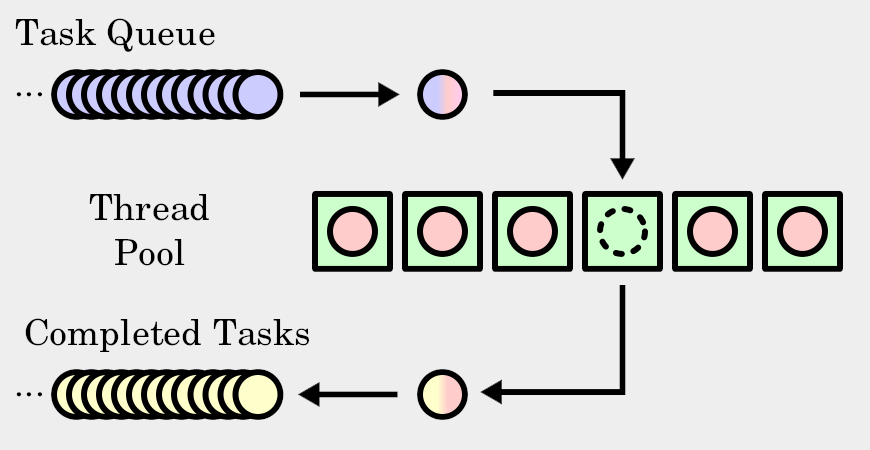
\includegraphics[height=6cm]{img/threadpool.png}
  \end{center}
\end{frame}

\begin{frame}[fragile]{Wątki}
\begin{columns}[T]
  \begin{column}{0.7\textwidth}
    \begin{itemize}
      \item{} \texttt{std::thread(\textit{Function} f, Args\&\&... args)}
      \item{} \texttt{join()} dołącza wątek do głównego wątku
      \item{} \texttt{detach()} dołącza* wątek do głównego wątku
      \item{} header \texttt{<thread>}. Wymagany \texttt{-std=c++11} lub nowszy.
      \item{} szybki przykład
    \end{itemize}
  \end{column}
  \begin{column}{0.25\textwidth}
    
\includegraphics[height=3cm]{img/bees.png}
  \end{column}
\end{columns}
\end{frame}

\begin{frame}[fragile]{Zadanie 0.}
0. Napisz program ,,Hello, World!''.
  \begin{itemize}
    \item{} Wypisanie tekstu powinno nastąpić w dedykowanym wątku (innym niż wątek główny).
    \item{} Sprawdź różnicę w działaniu metod \texttt{join()} i \texttt{detach()}.
  \end{itemize}
\end{frame}

\begin{frame}[fragile]{Zadanie 1.}
1. Przeanalizuj program \texttt{01.cpp}.
  \begin{itemize}
    \item{} Czy program jest \textcolor{yellow}{deterministyczny}?
    \item{} Dlaczego wewnątrz procedury \texttt{run()} korzystamy z klasy \texttt{string}?
    \item{} Jak zapewnić naprzemienność pracy wątków roboczych?
  \end{itemize}
\end{frame}

\begin{frame}[fragile]{Zadanie 2.}
2. Przeanalizuj program \texttt{02.cpp}.
  \begin{itemize}
    \item{} Czy program jest \textcolor{yellow}{deterministyczny}?
    \item{} Jak często wątki usiłują uzyskać dostęp do strefy krytycznej?
    \item{} Czy dostrzegasz potencjalne problemy tego kodu?
  \end{itemize}
\end{frame}

\begin{frame}[fragile]{Koniec}
  \begin{center}
    {\huge Dzięki za uwagę!}
  \end{center}
\end{frame}

\end{document}
